\documentclass[12pt]{report}
\usepackage{graphicx} 
\usepackage{float} 
\usepackage{subfigure} 
\usepackage{titlesec}
\usepackage{amsfonts,amsmath,amssymb,amsthm,geometry,bbm,hyperref,nicefrac,enumerate,comment}
\usepackage{mathabx}
\usepackage[shortlabels]{enumitem}

\titleformat{\chapter}[display]
  {\Huge\bfseries}{}{0pt}{\thechapter.\ }

\titleformat{name=\chapter,numberless}[display]
  {\Huge\bfseries}{}{0pt}{}
  

% \theoremstyle{plain}
\newtheorem{theorem}{Theorem}[chapter]

\newtheorem{example}[theorem]{Example} 
\newtheorem{corollary}[theorem]{Corollary}
\newtheorem{lemma}[theorem]{Lemma}
\newtheorem{proposition}[theorem]{Proposition}
\newtheorem{setting}[theorem]{Setting} 


\theoremstyle{definition}
\newtheorem{definition}[theorem]{Definition} 

\theoremstyle{remark}
\newtheorem*{remark}{Remark}

\newtheorem{mydef}{Definition}

\usepackage{bm}
\usepackage{mathrsfs}
\newcommand{\R}{\mathbb{R}}
\newcommand{\N}{\mathbb{N}}
\newcommand{\E}{\mathbb{E}}
\newcommand{\smallsum}{\textstyle\sum}
\renewcommand{\P}{\mathbb{P}}

\DeclareMathOperator*{\argmin}{arg\,min}
\DeclareMathOperator*{\argmax}{arg\,max}


\begin{document}

\begin{titlepage}
   \begin{center}
       \LARGE
       \textbf{A Study of Data-driven Market Simulator}
       \\
       \vspace{2cm}
       \Large Master Thesis
 
       \vspace{1.5cm}

       \Large
       Songyan Hou\\
 
       \vfill

       
       \textit{\large Supervisor:}\\
       \large

       Prof. Dr. Josef Teichmann\\
       \normalsize
       Department of Mathematics\\
       ETH Z\"urich\\

       \vspace{0.8cm}
       Submitted: \today
 
   \end{center}
\end{titlepage}

\begin{abstract}
  asd
\end{abstract}

\tableofcontents
\chapter{Introduction}

\chapter{Financial times-series stimulation}
\section{Challenges in financial scenario}
\section{Stylized facts and evaluation of similarity}
\section{Classical and modern model}

\chapter{Signature feature}
In this chapter, we give a brief introduction to the signature feature of a path and some variation of signature feature such as log-signature, low-rank-signature and random-signature. Moreover, we discuss the expectation of these signature based features of a stochastic process and emphasize their characteristic ability of the law of stochastic process. For simplicity and readability, we restrict our introduction to the space of continuous bounded variation paths from a compact time interval $J$ to a Euclidean space $E = \R^{d}$ denoted by $\mathcal{C}^{1}_{0}(J,E)$. We postpone the discussion of semi-martingales and rough paths taking values in Banach space $E$ to the appendix and kindly invite interested readers to the comprehensive and rigorous introduction of signature feature in \cite{friz2020course} \cite{lyons2007differential}.  

\section{Signature}
We start the introduction from the tensor algebra in which our signature feature takes value. We consider the non-commuting formal power series of tensors with formal indeterminates as basis of $E$. 
\begin{definition}[Formal power series]
  We denote $T((E))$ the space of formal power series of tensors in $E$ that 
  \begin{equation}
    \begin{split}
      T((E)) &= \Bigg\{\mathbf{a} = (\mathbf{a}_{k})_{k\geq 0} \colon \mathbf{a}_{k} \in E^{\otimes k}\Bigg\} = \bigoplus_{m\geq 0} E^{\otimes m} \\
    \end{split}
  \end{equation}
  endowed with addition and multiplication defined as follows: Let $\mathbf{a} = (\mathbf{a}_{k})_{k\geq 0}, \mathbf{b} = (\mathbf{b}_{k})_{k\geq 0} \in T((E))$ and $\lambda \in \R$. Then 
\begin{equation}
  \begin{split}
    \mathbf{a} + \mathbf{b} &= (\mathbf{a}_{k} + \mathbf{b}_{k})_{k\geq 0}\\
    \mathbf{a} \otimes \mathbf{b} &= \big(\sum_{i+j = k}\mathbf{a}_{i} \otimes \mathbf{b}_{j}\big)_{k\geq 0}\\
    \lambda\mathbf{a} &= (\lambda \mathbf{a}_{k})_{k\geq 0}
  \end{split}
\end{equation}
Let $T^{(n)}(E)$ denote the truncated tensor algebra space up to order $n$
\begin{equation}
  T^{(n)}(E) = \bigoplus_{k\leq n} E^{\otimes k}
\end{equation}  
\end{definition}
Let $e_{1},\cdots,e_{d}$ be a finite basis of $E = \R^{d}$. Then $\mathbf{a}\in T((E))$ has the following linear form
\begin{equation} 
  \mathbf{a} = \sum_{k\geq 0}\Big(\sum_{i_{1},\cdots,i_{k} = 1}^{d} a_{i_{1},\cdots,i_{k}}e_{i_{1}}\otimes\cdots\otimes e_{i_{k}} \Big),\quad a_{i_{1},\cdots,i_{k}} \in \R.
\end{equation}
and $T^{(n)}(E)$ can be considered as a subspace of $T((E))$.
% and $T((E))$ is endowed with inner product naturally inherited from $\R^{d}$. 
% \begin{equation}
%   \langle e_{i_{1}}\otimes\cdots\otimes e_{i_{k}}, e_{j_{1}}\otimes\cdots\otimes e_{j_{k}} \rangle_{T((E))} = \delta_{i_{1},j_{1}}\cdots \delta_{i_{k},j_{k}}
% \end{equation} 

\begin{definition}
  We denote $\mathbf{T}(E)$ the Banach space 
  \begin{equation}
    \mathbf{T}(E) \coloneq \bigg\{\mathbf{t} \in T((E)) \colon \lVert \mathbf{t}\rVert_{\mathbf{T}(E)} \coloneq \sqrt{\sum_{k\geq 0}\lVert \mathbf{t}_{k}\rVert_{E^{\otimes k}}^{2} } < \infty \bigg\}.
  \end{equation} 
  Similarly, we denote $\mathbf{T}^{(n)}(E)$ the truncation of $\mathbf{T}(E)$ up to order $n$.
\end{definition}

\begin{definition}[Signature]
  We denote $\mathbf{Sig}_{J} \colon \mathcal{C}^{1}_{0}(J,E) \to \mathbf{T}(E)$ the signature map such that for all $X \in \mathcal{C}^{1}_{0}(J,E)$
  \begin{equation}
    \mathbf{Sig}_{J}(X) = (1, \mathbf{s}_{1},\cdots) \in \mathbf{T}(E)
  \end{equation}
  where 
  \begin{equation}
    \begin{split}
      \mathbf{s}_{k} &= \int_{t_{1}<\cdots< t_{k} \in J}dX_{t_{1}}\otimes\cdots\otimes dX_{t_{k}}\\
      &= \sum_{i_{1},\cdots,i_{k} = 1}^{d} \int_{t_{1}<\cdots< t_{k} \in J}dX_{t_{1}}^{i_{1}}\cdots dX_{t_{k}}^{i_{k}} \cdot e_{i_{1}}\otimes\cdots\otimes e_{i_{k}} \\
    \end{split}
  \end{equation}
  Let $\mathbf{Sig}^{(n)}_{J}$ denote the truncated signature map up to order $n$
  \begin{equation}
    \mathbf{Sig}^{(n)}_{J}(X) = (1, \mathbf{s}_{1},\cdots, \mathbf{s}_{M}) \in \mathbf{T}^{(n)}(E).
  \end{equation}
\end{definition}
\begin{example}\label{linear}
  Let $X_{t} = t\mathbf{x} \in \R^{d}$, then 
  \begin{equation}
    \mathbf{Sig}_{[0,1]}(X) = (1, \mathbf{x},\frac{\mathbf{x}^{\otimes 2}}{2!}, \cdots) \in \mathbf{T}(E)
  \end{equation}
\end{example}

\subsection{Signature map}
We expect a good feature map to capture important information while ignoring irrelevant ones. First observation is the the signature feature is invariant of starting point because $d(X_{t} - X_{0}) = dX_{t}$. Moreover, it is invariant of reparametrization.
\begin{proposition}[Invariant under reparametrization]
  Let $X \in \mathcal{C}^{1}_{0}([S_{1},T_{1}],E)$ and  $\tau\colon [S_{1},T_{1}] \to [S_{2},T_{2}]$ a non-decreasing surjective reparametrization. Then 
  \begin{equation}
    \mathbf{Sig}_{[S_{2},T_{2}]}(X_{\tau(\cdot)}) = \mathbf{Sig}_{[S_{1},T_{1}]}(X) 
  \end{equation}
\end{proposition}
\begin{proof}
  \begin{equation}
    \begin{split}
      \mathbf{Sig}_{[S_{2},T_{2}]}(X_{\tau(\cdot)})_{k} &= \int_{\tau(t_{1})<\cdots< \tau(t_{k}) \in [S_{2},T_{2}]}dX_{\tau(t_{1})}\otimes\cdots\otimes dX_{\tau(t_{k})}\\
      &= \int_{t_{1}<\cdots< t_{k} \in [S_{1},T_{1}]}dX_{t_{1}}\otimes\cdots\otimes dX_{t_{k})} = \mathbf{Sig}_{[S_{1},T_{1}]}(X) 
    \end{split}
  \end{equation}
\end{proof}
From the invariant property of reparametrization, we notice that signature map is not injective. However, signature feature is injective up to tree-like equivalence $\sim_{t}$ which we detailed in appendix, and obviously time-reparametrization is included in tree-like equivalence. We define $\mathcal{P}_{0}^{1} = \mathcal{C}^{1}_{0}([0,T],E) / \sim_{t}$ the quotient space up to tree-like equivalence endowed with quotient metric.  
\begin{theorem}[Weak uniqueness \cite{boedihardjo2016signature}] 
  $\mathbf{Sig}_{[0,T]}$ is injective on $\mathcal{P}_{0}^{1}$.
\end{theorem}
\begin{proof}
  See \cite{boedihardjo2016signature}.
\end{proof}
If we add time as an additional strictly increasing coordinate into path ie. $\overline{X_{t}} = (t,X_{t}) \in \overline{E} \coloneq \R\oplus E$, then $\mathbf{Sig}_{[0,T]}$ is injective on the time-augmented space. 
\begin{corollary}[Uniqueness \cite{boedihardjo2016signature}] 
  $\mathbf{Sig}_{[0,T]}$ is injective on $\mathcal{C}^{1}_{0}([0,T],\overline{E})$.
\end{corollary}
\begin{proof}
  Since the first coordinate is strictly increasing, the only tree-like equivalent path is itself i.e. $\mathcal{P}^{1}_{0} = \mathcal{C}^{1}_{0}([0,T],\overline{E})$, which concludes the proof. 
\end{proof}
\begin{proposition}\label{surjective}
  $\mathbf{Sig}_{[0,1]}$ is neither surjective nor the range of which a linear subspace of $\mathbf{T}(E)$.
\end{proposition}
\begin{proof}
  Let $X \in \mathcal{C}^{1}_{0}([0,T],E)$ and w.l.o.g assume $X_{0} = 0$. 
  By integration by part
  \begin{equation}
    \begin{split}
      \mathbf{Sig}_{[0,1]}(X)_{1,2} + \mathbf{Sig}_{[0,1]}(X)_{2,1} &=  \int_{t_{1}<t_{2} \in [0,1]}dX_{t_{1}}^{1}dX_{t_{2}}^{2} + \int_{t_{1}<t_{2} \in [0,1]}dX_{t_{1}}^{1}dX_{t_{2}}^{2}\\
      &=  \int_{t \in [0,1]}d(X_{t}^{1}X_{t}^{2}) = \mathbf{Sig}_{[0,1]}(X)_{1}~\mathbf{Sig}_{[0,1]}(X)_{2}.
    \end{split}
  \end{equation}
  Thus, $\mathbf{Sig}_{[0,1]}$ is neither surjective nor the range of it a linear subspace of $\mathbf{T}(E)$.
\end{proof}

\begin{theorem}[Weak universality]
  Let $A$ be a compact set of $\mathbf{Sig}(\mathcal{C}^{1}_{0}(J,E))$, then for all $f \colon A \to \R$ continuous and for all $\epsilon > 0$, there exists a linear functional $L \in \mathbf{T}(E)^{*}$ such that 
  \begin{equation}
    \sup_{\mathbf{a}\in A}\lVert f(\mathbf{a}) - L(\mathbf{a})\rVert \leq \epsilon
  \end{equation}
\end{theorem}
\begin{proof}
  Proof relies on the Stone-Weierstrass theorem and the shuffle product property of the signature detailed in appendix, see \cite{liao2019learning}.
\end{proof}


\subsection{Signature stream}
Instead of viewing signature as a static object, we can consider signature stream of a path $X \in \mathcal{C}^{1}_{0}([0,T],E)$ as a process $\big(\mathbf{Sig}_{[0,t]}(X)\big)_{[0,T]}$ taking values in $\mathbf{T}(E)$.
\begin{proposition}
  Let $X \in \mathcal{C}^{1}_{0}([0,T],E)$ and define $\pi_{n} \colon \mathbf{T}(E) \to \mathbf{T}^{(n)}(E)$ the projection such that for all $\mathbf{x} \in \mathbf{T}(E)$ 
  \begin{equation}\label{projection}
    \pi_{n}\big((\mathbf{x}_{k})_{k\geq 0}\big) = (\mathbf{x}_{k})_{k\leq n}
  \end{equation}
  then $S_{t} = \mathbf{Sig}^{(n)}_{[0,t]}(X)$ satisfies for all $t \in [0,T]$ that 
  \begin{equation}\label{SDE_signature}
    dS_{t} = \pi_{n}(S_{t}\otimes dX_{t}),\quad S_{0} = (1,0,\cdots),
  \end{equation} 
  and moreover $(S_{t})_{t \in [0,T]}$ is the unique solution of \eqref{SDE_signature}. 
\end{proposition}
\begin{proof}
  See Lemma 2.10 in \cite{lyons2007differential}.
\end{proof}


\begin{definition}
  Let $X \in \mathcal{C}^{1}_{0}([0,s],E)$ and  $X \in \mathcal{C}^{1}_{0}([s,t],E)$. The concatenated path $X\star Y \in\mathcal{C}^{1}_{0}([0,t],E) $ is defined by 
  \begin{equation}
    (X\star Y)_{u} = \left\{\begin{aligned}
      &X_{u} &u\in [0,s]\\
      &Y_{u} + (X_{s} - Y_{s}) &u\in [s,t]
    \end{aligned}\right.
  \end{equation}
\end{definition}
\begin{theorem}[Chen's identity]
  Let $X \in \mathcal{C}^{1}_{0}([0,s],E)$ and  $Y \in \mathcal{C}^{1}_{0}([s,t],E)$. Then 
  \begin{equation}
    \mathbf{Sig}_{[0,t]}(X\star Y) = \mathbf{Sig}_{[0,s]}(X) \otimes \mathbf{Sig}_{[s,t]}(Y)
  \end{equation}
\end{theorem}
\begin{proof}
  See Theorem 2.9 in \cite{lyons2007differential}.
\end{proof}

\begin{example}\label{linear_chern}
  Let $X$ be linear on $[n,n+1]$ and let $X_{n+1} - X_{n} = \mathbf{x}_{n}$ for $n \in \N$, then 
  \begin{equation}
    \mathbf{Sig}_{[0,N]}(X) = \bigotimes_{n \leq N}(1, \mathbf{x}_{n},\frac{\mathbf{x}_{n}^{\otimes 2}}{2!}, \cdots) 
  \end{equation}
\end{example}


\begin{example}[Linear controlled differential equation]\label{lcde}
  Let $E = \R^{d}, W = \R^{n}$. let $X \in \mathcal{C}^{1}_{0}([0,T],E)$ and let $B\colon E \to \mathbf{L}(W)$ be a bounded linear map. Consider 
  \begin{equation}
    dY_t = B(dX_{t})(Y_{t}),\quad Y_{0} \in W  
  \end{equation}
  If we denote $B^{k} \coloneq B(e_{k})$, $k = 1,\cdots, d$ then 
  \begin{equation}\label{linear_control}
    dY_t = \sum_{k=1}^{d}B^{k}(Y_{t})dX^{k}_{t},\quad Y_{0} \in W .
  \end{equation}
  It follows from Picard's iteration that 
  \begin{equation}
    \begin{split}
      Y^{n}_{t} &= \Bigg(I + \sum_{k=1}^{n}B^{\otimes k}\int_{t_{1}<\cdots< t_{k} \in [0,t]}dX_{t_{1}}\otimes\cdots\otimes dX_{t_{k}}\Bigg) Y_{0}\\ 
      &= \Bigg(I + \sum_{k=1}^{n}\sum_{i_{1},\cdots,i_{k} = 1}^{d}B^{i_{k}}\cdots B^{i_{1}}\int_{t_{1}<\cdots< t_{k} \in [0,t]}dX_{t_{1}}^{i_{1}}\cdots dX_{t_{k}}^{i_{k}}\Bigg) Y_{0}.
    \end{split}
  \end{equation}
  Let the variation of $X \in \mathcal{C}^{1}_{0}([0,T],E)$ denoted by $\lVert X \rVert_{[0,T]}$, then 
  \begin{equation}
      \Big\lVert \int_{t_{1}<\cdots< t_{k} \in [0,t]}dX_{t_{1}}\otimes\cdots\otimes dX_{t_{k}} \Big\rVert_{E^{\otimes k}} \leq \frac{\lVert X \rVert_{[0,T]}^{k}}{k!}.
  \end{equation}
  Therefore, $Y^{n}_{t}$ converges to $Y_{t}$ as $n \to \infty$ i.e. 
  \begin{equation}
    \lVert Y_{t} - Y^{n}_{t}\rVert_{W} \leq \sum_{k > n}\frac{\lVert B\rVert_{\mathcal{L}(E,\mathcal{L}(W))}^{k}\lVert X \rVert_{[0,T]}^{k}}{k!}  \leq \frac{\lVert B\rVert_{\mathcal{L}(E,\mathcal{L}(W))}^{n+1}\lVert X \rVert_{[0,T]}^{n+1}}{n!} \to 0,\quad \text{as } n \to \infty
  \end{equation}
  and
  \begin{equation} 
    Y_{t} = \Bigg(I + \sum_{k=1}^{\infty}B^{\otimes k}\int_{t_{1}<\cdots< t_{k} \in [0,t]}dX_{t_{1}}\otimes\cdots\otimes dX_{t_{k}}\Bigg) Y_{0}.
  \end{equation}
  In the language of signature 
  \begin{equation} 
    Y_{t} = \Big(\sum_{k=0}^{\infty}B^{\otimes k}\Big) \Big(\mathbf{Sig}_{[0,t]}(X)\Big) Y_{0}.
  \end{equation}
  which implies that the solution of controlled SDE could be written as a linear function on signature stream of control path. This implies that signature stream is a promising feature for controlled ODE.
\end{example}
\begin{remark}
  Similar result holds for smooth vector field with some additional boundness assumption and the proof is in alignment with the argument above, see \cite{liao2019learning}. 
\end{remark}
Despite nice properties as feature map, signature feature suffers from dimension explosion w.r.t truncation order. Consider a path $X \in \mathcal{C}^{1}_{0}([0,T],\R^{d})$ and the truncated signature of $X$ up to order $n$ in $\mathbf{T}^{(n)}(\R^{d}) \subseteq \bigoplus_{k\leq n} (\R^{d})^{\otimes k} $ which has dimension $1 + d + \cdots + d^{n} = \frac{d^{n+1} - d}{d-1}$ growing exponentially w.r.t the truncation order $n$. Therefore, we would like to explore some low-rank approximations of signature feature. 
\section{Log-signature}
From Proposition \ref{surjective}, we know that $\mathbf{Sig}_{[0,1]}$ is neither surjective nor the range of which a linear subspace of $\mathbf{T}(E)$. In Example \ref{linear}, for $X_{t} = t\mathbf{x} \in \R^{d}$, then 
  \begin{equation}
    \mathbf{Sig}_{[0,1]}(X) = \sum_{k\geq 0}\frac{\mathbf{x}^{\otimes k}}{k!}
  \end{equation}
  which is the power series expansion of exponential function. Motivated by this, we curve the signature space by taking `logarithm' which we defined below. 
\begin{definition}
  Define $\mathbf{T}_{1}(E) = \{\mathbf{a} \in \mathbf{T}(E)\colon \mathbf{a}_{0} = 1\}$. Let $\mathbf{a} \in \mathbf{T}_{1}(E)$, we define the exponential be 
  \begin{equation}
    \mathbf{exp}(\mathbf{a}) = \sum_{n\geq 0}\frac{\mathbf{a}^{\otimes n}}{n!}.
  \end{equation}
  and we define the logarithm be
  \begin{equation}
    \mathbf{log}(\mathbf{a}) = \mathbf{log}(1+\mathbf{t}) = \sum_{n\geq 1} \frac{(-1)^{n-1}}{n}\mathbf{t}^{\otimes \mathbf{n}}.
  \end{equation}
\end{definition}
\begin{lemma}
  $\mathbf{exp}(\cdot)$ and $\mathbf{log}(\cdot)$ are inverse of each other on $\mathbf{T}_{1}(E)$.
\end{lemma}
\begin{proof}
  See Lemma 2.21 in \cite{lyons2007differential}.
\end{proof}
Therefore, taking logarithm of signature loses no information.
\begin{definition}[Log-signature]
  We denote $\mathbf{LogSig}_{J} \colon \mathcal{C}^{1}_{0}(J,E) \to \mathbf{T}(E)$ the log-signature map such that for all $X \in \mathcal{C}^{1}_{0}(J,E)$
  \begin{equation}
    \mathbf{LogSig}_{J}(X) = \mathbf{log}\big(\mathbf{Sig}_{J}(X)\big)
  \end{equation}
  Let $\mathbf{LogSig}^{(n)}_{J}$ denote the truncated signature map up to order $n$
  \begin{equation}
    \mathbf{LogSig}^{(n)}_{J}(X) = \pi_{n}\big(\mathbf{LogSig}_{J}(X)\big)
  \end{equation}
  where $\pi_n$ define in \eqref{projection}.
\end{definition}
\subsection{Lie Series}
Besides storing the same information, thanks to the shuffle product property of signature, log-signature space is linear and admits a more concrete representation. Precisely speaking, log-signature space is a linear subspace of Lie formal series over $E$. Recall the Lie bracket $[\cdot, \cdot]$ on $T((E))$ such that 
\begin{equation}
  [\mathbf{a},\mathbf{b}] = \mathbf{a}\otimes\mathbf{b} - \mathbf{b}\otimes\mathbf{a}
\end{equation}
If $F_{1}$ and $F_2$ are two linear subspaces of $T((E))$, let us denote by $[F1, F2]$ the linear span of all the elements of the form $[\mathbf{a}, \mathbf{b}]$, where $\mathbf{a} \in F_{1}$ and $\mathbf{b} \in F_{2}$.
\begin{definition}[Lie formal series]
  We denote $\mathcal{L}((E))$ the space of Lie formal series over $E$ such that 
  \begin{equation}
    \mathcal{L}((E)) = \{\mathbf{l} \in T((E)) \colon \mathbf{l}_{n} \in L_{n}\}
  \end{equation} 
  where 
  \begin{equation}
    L_{0} = 0, L_{1} = [E,E], L_{2} = [E,L_{1}], \cdots ,L_{n} = [E,L_{n-1}], \cdots
  \end{equation}
  and denote $\mathcal{L}^{(n)}(E) = \pi_{n}(\mathcal{L}((E)))$ the truncated Lie series up to order $n$.
\end{definition}
\begin{theorem}
  The range of log-signature is a linear subspace of Lie series over $E$.
  \begin{equation}
    \mathbf{LogSig}(\mathcal{C}_{0}^{1})\subseteq\mathcal{L}((E)).
  \end{equation}
\end{theorem}
\begin{proof}
  See Theorem 2.23 in \cite{lyons2007differential}.
\end{proof}
\begin{theorem}\label{truncatedLieseries}
  The range of truncated log-signature is the truncated Lie series over $E$ up to the same order
  \begin{equation}
    \mathbf{LogSig}^{(n)}(\mathcal{C}_{0}^{1}) = \mathcal{L}^{(n)}(E)
  \end{equation}
\end{theorem}
\begin{proof}
  See Proposition 2.27 in \cite{lyons2007differential}.
\end{proof}
With Lie series form, we compute the dimension of truncated log-signature space. 
\begin{proposition}\label{logsignatureorder}
  The dimension of the space of truncated log-signature up to order $n$ is 
  \begin{equation}
    w(d,n) = \sum_{k=1}^{n}\frac{1}{k}\sum_{i|k}\mu\Big(\frac{k}{i}\Big)d^{i}
  \end{equation}
  which is the Witt's formula and $\mu$ is the M\"{o}bius function.
\end{proposition}
\begin{proof}
  See Corollary 4.14 in \cite{reutenauer2003free}.
\end{proof}
If we let $d=5$ and $n=5$, then $\dim(\mathbf{Sig}) = 3905$ while $\dim(\mathbf{LogSig}) = 829$. In summary, log-signature curves the signature space and reduces the redundancy without losing any information. However, there is no free lunch because log-signature loses the universality of signature, therefore requiring nonlinear models.  
\begin{example}
  For $X_{t} = t\mathbf{x} \in \R^{d}$, then 
  \begin{equation}
    \mathbf{Sig}_{[0,1]}(X) = \mathbf{exp}(\mathbf{x}),\quad \mathbf{LogSig}_{[0,1]}(X) = \mathbf{x}.
  \end{equation}
  Log-signature pick non-redundant information in signature.  
\end{example}
\section{Universality and characteristics }
Recall the weak universality of signature, we restrict ourselves on a compact set of $\mathbf{Sig}(\mathcal{C}^{1}_{0}(J,E))$. To generalize the theorem beyond compactness, we would like to normalize the set $\mathbf{Sig}(\mathcal{C}^{1}_{0}(J,E))$ into a bounded ball. The first idea comes to mind is to normalize signatures by scaling them on $\mathbf{T}(E)$. However, because signature map is neither surjective nor the range of it a linear subspace, scaled tensor of a signature might not be signature. Thus, we drive ourselves out of the region of $\mathbf{Sig}(\mathcal{C}^{1}_{0}(J,E))$ where we have the shuffle product property. An alternative is to normalize the signature by scaling the path. For $X \in \mathcal{C}^{1}_{0}(J,E)$ and $\lambda > 0$, the signature of the scaled path
\begin{equation}
  \begin{split}
    \mathbf{Sig}_{J}(\lambda X)_{k} &= \int_{t_{1}\leq\cdots\leq t_{k} \in J}d\lambda X_{t_{1}}\otimes\cdots\otimes d\lambda  X_{t_{k}}\\ 
    &= \lambda^{k}\int_{t_{1}\leq\cdots\leq t_{k} \in J}dX_{t_{1}}\otimes\cdots\otimes dX_{t_{m}} = \lambda^{k}\mathbf{Sig}_{J}(X)_{k}
  \end{split}
\end{equation}
Thus, the norm of the scaled path
\begin{equation}
  \begin{split}
    \big\lVert \mathbf{Sig}_{J}(\lambda X)\big\rVert_{\mathbf{T}(E)}^{2} &= \sum_{k\geq 0} \lambda^{2k} \lVert \mathbf{Sig}_{J}(X)_{k}\rVert_{E^{\otimes k}}^{2} \\
    % &\neq \lambda \sqrt{\sum_{k\geq 0}\lVert \mathbf{Sig}_{J}(X)_{k}\rVert_{E^{\otimes k}}^{2} } = \lambda\big\lVert \mathbf{Sig}_{J}( X)\big\rVert_{\mathbf{T}(E)}\\
  \end{split}
\end{equation}
Therefore, we define the scaling map $\delta_{\lambda}$ on $\mathbf{T}(V)$ such that for all $\mathbf{a} \in \mathbf{T}(V)$ 
\begin{equation}
  \delta_{\lambda}(\mathbf{a}) = (\lambda^{k} \mathbf{a}^{k})_{k\geq 0}
\end{equation} 
\begin{definition}
  A tensor normalization is a continuous injective map 
  \begin{equation}
    \Lambda\colon \mathbf{T}(V) \to \{\mathbf{t} \in \mathbf{T}(V)\colon \lVert\mathbf{t}\rVert_{\mathbf{T}(E)} \leq K\}
  \end{equation}
  \begin{equation}
    \mathbf{t} \mapsto \delta_{\lambda(\mathbf{t} )}(\mathbf{t} )
  \end{equation}
  where $K > 0$ and $\lambda\colon \mathbf{T}(V) \to (0,\infty)$ a function. 
\end{definition}
The existence of tensor normalization is not trivial because of the nonlinear relationship between the scaling factor $\lambda(\mathbf{t})$ and the norm of scaled tensor $\lVert \delta_{\lambda(\mathbf{t} )}(\mathbf{t} ) \rVert $ shown above. The proof of existence and the construction methodology can be found in the appendix. 
\begin{theorem}[\cite{chevyrev2018signature}]\label{moment_law}
  Let $\Lambda \colon \mathbf{T}(E) \to \mathbf{T}(E)$ be a tensor normalization. The normalized signature 
  \begin{equation}
    \Phi = \Lambda \circ \mathbf{Sig}_{J}
  \end{equation}
  \begin{enumerate}[(i)]
    \item is a continuous injection from $\mathcal{P}_{0}^{1}$ in to a bounded subset of $\mathbf{T}(E)$,
    \item is universal to $C_{b}(\mathcal{P}_{0}^{1},\R)$, equipped with the strict topology, 
    \item is characteristic to the space of finite regular Borel measures on $\mathcal{P}_{0}^{1}$.
  \end{enumerate}
\end{theorem}  
\begin{proof}
  See Proposition 4.1 in \cite{chevyrev2018signature}.
\end{proof}
\begin{corollary}\label{equalequal}
  Let $X$ a stochastic process on $[0,1]$ and measurable $(\Omega,\mathcal{F})$. Let $\P$ and $\mathbb{Q}$ be two regular probability measures such that $X \in \mathcal{P}_{0}^{1}$ almost surely. Then 
  \begin{equation}
    \E_{\P}[\Phi(X)] = \E_{\mathbb{Q}}[\Phi(X)]\quad\text{iff}\quad \P = \mathbb{Q}
  \end{equation} 
\end{corollary}
\begin{proof}
 Proof directly from (iii) of Theorem \ref{moment_law}.
\end{proof}
\begin{remark}
  If we consider the regular probability measure on time augmented path space $\mathcal{C}^{1}_{0}([0,T],\overline{E})$, similar result holds since $\mathcal{C}^{1}_{0}([0,T],\overline{E}) = \mathcal{P}_{0}^{1}$.
\end{remark}

\begin{definition}[Maximum mean distance]
  We define the maximum mean distance (MMD) as 
  \begin{equation}
    d_{\mathcal{G}}(\P,\mathbb{Q}) = \sup_{f\in\mathcal{G}}\lvert \E_{\P}[f] - \E_{\mathbb{Q}}[f]\rvert 
  \end{equation}
  where $\mathcal{G} \subseteq \R^{\mathcal{P}_{0}^{1}}$.
\end{definition}
Let $ \mathcal{G} = \{\langle\mathbf{l},\Phi(\cdot)\rangle_{\mathbf{T}_{1}} \colon \mathbf{l} \in \mathbf{T}_{1}, \lVert \mathbf{l}\rVert_{\mathbf{T}_{1}} \leq 1\}$, then by Corollary \ref{equalequal}
\begin{equation}
  d_{\mathcal{G}}(\P,\mathbb{Q}) = 0\quad\text{iff}\quad \P = \mathbb{Q}
\end{equation}
which implies that  a metric, see \cite{1993Probability}. Moreover 
\begin{equation}
  \begin{split}
    d_{\mathcal{G}}(\P,\mathbb{Q}) &= \sup_{f\in\mathcal{G}}\lvert \E_{\P}[f] - \E_{\mathbb{Q}}[f]\rvert \\
    &= \sup_{f\in\mathcal{G}}\Big\lvert \E_{(X,Y) \sim \P\otimes\mathbb{Q}}[f(X) - f(Y)]\Big\rvert \\  
    &= \sup_{\mathbf{l} \in \mathbf{T}_{1}, \lVert \mathbf{l}\rVert_{\mathbf{T}_{1}} \leq 1}\Big\lvert \E_{(X,Y) \sim \P\otimes\mathbb{Q}}\big[\langle \mathbf{l}, \Phi(X) - \Phi(Y)\rangle_{\mathbf{T}_{1}}\big]\Big\rvert \\  
  \end{split}
\end{equation}
Since $\E_{(X,Y) \sim \P\otimes\mathbb{Q}}\big[\Phi(X) - \Phi(Y)\big] \in \mathbf{T}_{1}$, then 
\begin{equation}\label{eq348}
  \begin{split}
    d_{\mathcal{G}}(\P,\mathbb{Q}) &= \E\big[\langle \Phi(X) - \Phi(Y), \Phi(X^{\prime}) - \Phi(Y^{\prime})\rangle_{\mathbf{T}_{1}}\big]\\
  \end{split}
\end{equation}
where $X,Y,X^{\prime},Y^{\prime}$ are independent with $X,X^{\prime}\sim\P$ and $Y,Y^{\prime}\sim\mathbb{Q}$
\begin{definition}
  We denote $\mathbf{k_{Sig}}\colon \mathbf{T}_{1}\times\mathbf{T}_{1} \to \R$ the signature kernel such that 
  \begin{equation}
    \mathbf{k_{Sig}}(\cdot,\cdot) = \langle \Phi(\cdot),\Phi(\cdot)\rangle_{\mathbf{T}_{1}}
  \end{equation}
\end{definition}
Then we can rewrite the MMD as 
\begin{equation}
   d_{\mathcal{G}}(\P,\mathbb{Q}) = \E\big[\mathbf{k_{Sig}}(X,X^{\prime})\big] - 2\E\big[\mathbf{k_{Sig}}(X,Y)\big] + \E\big[\mathbf{k_{Sig}}(Y,Y^{\prime})\big]
\end{equation}
where $X,Y,X^{\prime},Y^{\prime}$ are independent with $X,X^{\prime}\sim\P$ and $Y,Y^{\prime}\sim\mathbb{Q}$. Similar to the kernel trick in machine learning, the kernel representation of MMD provides a very efficient way evaluating the metric, which we will elaborate in the next section.  





\section{Discrete signature feature}
Let $X \in \mathcal{C}^{1}_{0}([0,1],E)$ and consider a discrete sequence $\mathbf{X} = (X_{0},X_{1/N},\cdots, X_{1}) \in E^{N+1}$. We extend the concept of signature on discrete sequence $E^{N+1}$ by computing signature of the linear interpolation of sequence. From Example \ref{linear_chern} we know the signature of piecewise-linear path is 
\begin{equation}
  \mathbf{exp}(\mathbf{X}_{1} - \mathbf{X}_{0}) \otimes \cdots \otimes \mathbf{exp}(\mathbf{X}_{N} - \mathbf{X}_{N-1})
\end{equation}
Therefore we define the discrete signature as follows 
\begin{definition}
  Let $\mathbf{X} = (\mathbf{X}_{i})_{i=0}^{N} \in E^{N+1}$ and let $\triangle \mathbf{X}_{i} = \mathbf{X}_{i} - \mathbf{X}_{i-1}$. We denote $\mathbf{sig}_{[0,N]}$ the discrete signature of order $m$ and depth $n$ such that 
  \begin{equation}
    \mathbf{sig}_{[0,N]}(\mathbf{X}) = \pi_{n}\bigg(\bigotimes_{i=1}^{N}\pi_{m}\Big(\mathbf{exp}\big(\triangle \mathbf{X}_{i}\big)\Big)\bigg)
  \end{equation} 
\end{definition}
In particular, if $m = 1$ we call it growing discrete signature
  \begin{equation}
    \begin{split}
      \mathbf{sig}_{[0,N]}(\mathbf{X}) &= \pi_{n}\bigg(\prod_{i=1}^{N}\big(1 + \triangle \mathbf{X}_{i}\big)\bigg)\\
      &= \sum_{k=0}^{n}\sum_{i_{1} < \cdots < i_{k} = 1}^{N} \triangle \mathbf{X}_{i_{1}} \otimes \cdots \otimes \triangle \mathbf{X}_{i_{k}}.
    \end{split}
  \end{equation} 
  If $m > 1$, we call it high order discrete signature, and if $m \geq n$, we call it truncated discrete signature
  \begin{equation}
    \begin{split}
      \mathbf{sig}_{[0,N]}(\mathbf{X}) &= \pi_{n}\bigg(\prod_{i=1}^{N}\mathbf{exp}\big(\triangle \mathbf{X}_{i}\big)\bigg)\\
      &= \sum_{k=0}^{n}\sum_{i_{1} \leq \cdots \leq i_{k} = 1}^{N} \triangle \mathbf{X}_{i_{1}} \otimes \cdots \otimes \triangle \mathbf{X}_{i_{k}} 
    \end{split}
  \end{equation} 
  \begin{lemma}
    Let $X \in \mathcal{C}^{1}_{0}([0,1],E)$ and $\mathbf{X} = (X_{i/N})_{i=0}^{N} \in E^{N+1}$, then
    \begin{equation}
      \lVert \mathbf{Sig}_{[0,1]}(X) - \mathbf{sig}_{[0,N]}(\mathbf{X})\rVert_{\mathbf{T}_{1}} \to 0\quad\text{as}\quad N \to 0
    \end{equation}
  \end{lemma}
  \begin{proof}
    See Theorem 5 in \cite{kiraly2019kernels}.
  \end{proof}
  \begin{remark}
    If we let $X$ to be the Brownian motion (not in $\mathcal{C}^{1}_{0}$), the growing discrete signature converges to the signature defined with Ito integral, while the high order discrete signature converges to the signature defined with Stratonovich integral. More generally, if we want to approximate a geometric $p$-rough path, we need high order discrete signature at least order $\lfloor p \rfloor$, see \cite{kiraly2019kernels}.
  \end{remark}
  \subsection{Kernel trick}
  In the same fashion of horner algorithm 
  \begin{equation}
    \begin{aligned}a_{0}&+a_{1}x+a_{2}x^{2}+a_{3}x^{3}+\cdots +a_{n}x^{n}\\&=a_{0}+x{\bigg (}a_{1}+x{\Big (}a_{2}+x{\big (}a_{3}+\cdots +x(a_{n-1}+x\,a_{n})\cdots {\big )}{\Big )}{\bigg )}.\end{aligned}
  \end{equation}
  we can reduce the computational complexity of discrete signature by dynamic programming principle.
  \begin{proposition}Let $\mathbf{X} = (\mathbf{X}_{i})_{i=0}^{N} \in E^{N+1}$ and let $\mathbf{sig}_{[0,N]}$ be the growing signature
  \begin{equation}
    \begin{split}
      \mathbf{sig}_{[0,N]}(\mathbf{X}) &= \mathbf{sig}_{[0,N-1]}(\mathbf{X}) \otimes(1 + \triangle \mathbf{X}_{N})\\
      &= 1 + \sum_{i_{1} = 1}^{N}\triangle \mathbf{X}_{i_{1}}\Big(1 + \sum_{i_{2} = i_{1}+1}^{N}\triangle\mathbf{X}_{i_{2}}(\cdots)\Big)\\
    \end{split}
  \end{equation}
  \end{proposition}
  This is too surprise because we just rewrite the Chen's identity. However, this greatly reduce the complexity when computing the kernel. 
  \begin{definition} Let $\mathbf{sig}_{[0,N]}$ be the discrete signature, then we denote $\mathbf{k}_{\mathbf{sig}}$ the discrete signature kernel such that 
  \begin{equation}
    \mathbf{k}_{\mathbf{sig}}(\cdot,\cdot) = \langle \mathbf{sig}_{[0,N]}(\cdot),\mathbf{sig}_{[0,N]}(\cdot)\rangle_{\mathbf{T}_{1}}
  \end{equation}
  \end{definition}
  \begin{proposition}\label{recur1}
    Let $\mathbf{X} = (\mathbf{X}_{i})_{i=0}^{N} \in E^{N+1}$ and let $\mathbf{Y} = (\mathbf{Y}_{i})_{i=0}^{N} \in E^{N+1}$. Let $\mathbf{k}_{\mathbf{sig}}$ be the kernel of discrete growing signature
  \begin{equation}\label{kernel}
    \mathbf{k}_{\mathbf{sig}}(\mathbf{X},\mathbf{Y}) = 1 + \sum_{\substack{i_{1}=1 \\ j_{1} = 1}}^{N}\langle \triangle \mathbf{X}_{i_{1}},  \triangle \mathbf{Y}_{j_{1}} \rangle\Big(1 + \sum_{\substack{i_{2}=i_{1}+1 \\ j_{2} = j_{1}+1}}^{N}\langle \triangle \mathbf{X}_{i_{2}},  \triangle \mathbf{Y}_{j_{2}} \rangle(\cdots)\Big)
  \end{equation}
  \end{proposition}  
  \begin{remark}
    Similar formulas hold for high order discrete signature and kernel, see \cite{kiraly2019kernels}. 
  \end{remark}
  This result is important for numerical implementation in two aspects. First is that we avoid computing the tensor but the inner product directly by kernel trick. If somehow (for better characteristic capacity) you would like lift paths to a RKHS space $(H,\kappa)$ before applying the signature kernel, this formula avoids explicitly compute $\triangle\kappa_{X}$ and $\triangle\kappa_{Y}$. but approximating with
    \begin{equation}
      \langle\triangle\kappa_{X_{i}}, \triangle\kappa_{Y_{j}}\rangle\approx\kappa(X_{i+1},Y_{j+1}) + \kappa(X_{i},Y_{j}) - \kappa(X_{i},Y_{j+1}) - \kappa(X_{i+1},Y_{j}),
    \end{equation}
    which reduce a potentially infinite computational complexity if $(H,\kappa)$ is an infinite dimensional space, see \cite{chevyrev2018signature}. Secondly, the recursive structure in time implies that computing the inner product of signature stream is as cheap as computing the inner product of signature. This recursive feature can also be used for more general inner product between tensor and discrete signature. 

\section{Low-rank-signature}
We extend the recursive method from discrete signature to tensor with similar recursive structure. Let $\mathbf{l} = (\mathbf{l}_{k})_{k=0}^{\infty} \in \mathbf{T}_{1}(E)$, let $\mathbf{X} = (\mathbf{X}_{i})_{i=0}^{N} \in E^{N+1}$,and let $\mathbf{sig}_{[0,N]}$ be the growing signature. If $\mathbf{l}_{k} = \mathbf{l}_{k-1}\otimes l_{k}$ then
  \begin{equation}
    \begin{split}
     \langle \mathbf{l}, \mathbf{sig}_{[0,N]}(\mathbf{X}) \rangle_{\mathbf{T}_{1}(E)} &= \sum_{k\geq 0}\langle \mathbf{l}_{k} , \mathbf{sig}^{(k)}_{[0,N]}(\mathbf{X}) \rangle_{\mathbf{T}_{1}(E)} \\
     &= \sum_{k\geq 0}\sum_{i=1}^{N} \langle \mathbf{l}_{k-1} ,\mathbf{sig}^{(k-1)}_{[0,i-1]}(\mathbf{X})\rangle_{\mathbf{T}_{1}(E)}\cdot\langle l_{k},\triangle \mathbf{X}_{i}\rangle_{\mathbf{T}_{1}(E)} \\
     &= 1 + \sum_{\substack{i_{1}=1 \\ j_{1} = 1}}^{N}\langle l_{i_{1}},  \triangle \mathbf{X}_{j_{1}} \rangle\Big(1 + \sum_{\substack{i_{2}=i_{1}+1 \\ j_{2} = j_{1}+1}}^{N}\langle l_{i_{2}},  \triangle \mathbf{X}_{j_{2}} \rangle(\cdots)\Big)
    \end{split}
  \end{equation}
  This is exactly the formula \eqref{kernel} in Proposition \ref{recur1}. In the intermediate step of computing the inner product, we have obtained the value of $\langle \mathbf{l}_{k} , \mathbf{sig}^{(k)}_{[0,N]}(\mathbf{X}) \rangle_{\mathbf{T}_{1}(E)}$ for all $k$. Therefore, if we consider a sequence of $L$ many tensors such that $\mathbf{l}_{k} = \mathbf{l}_{k-1}\otimes l_{k}$, then we can leverage the recursive structure in order and compute their inner product with signature in linear computational complexity w.r.t $L$.
  \begin{remark}
    This result can also be generalized to higher order case by considering the recursive algorithm computing high order discrete signature and kernel, see \cite{kiraly2019kernels}. However, in the paper \cite{toth2020seq2tens} introducing low-rank tensor projection of ordered sequential data, only first order recursive structure is considered. We believe that higher order recursive structure also exists and we wish to prove this claim in further research. 
  \end{remark} 
  
  If we only assume $\mathbf{l}_{k} = l_{k,1} \otimes \cdots \otimes l_{k,k}$, then we lose the recursive in order, but still we have the recursive in time of discrete signature and the kernel trick.
    \begin{equation}
    \begin{split}
     \langle \mathbf{l}_{k}, \mathbf{sig}^{(k)}_{[0,N]}(\mathbf{X}) \rangle_{\mathbf{T}_{1}(E)} &= \sum_{i=1}^{N} \langle l_{k,1} \otimes \cdots \otimes l_{k-1,k} ,\mathbf{sig}^{(k-1)}_{[0,i-1]}(\mathbf{X})\rangle_{\mathbf{T}_{1}(E)}\cdot\langle l_{k,k},\triangle \mathbf{X}_{i}\rangle_{\mathbf{T}_{1}(E)} \\
    \end{split}
  \end{equation}
  
  \begin{definition}
    We call $\mathbf{l}  \in \mathbf{T}_{1}$ rank-1 tensor if
    \begin{equation}
      \mathbf{l} = l_{1} \otimes \cdots \otimes l_{k},\quad \text{for some  }k \geq 1
    \end{equation}
    % and we call a set of rank-1 tensor $L = \{\mathbf{l} \in \mathbf{T}_{1}\colon\mathbf{l}\text{ is rank-1}\}$ recursive tensors if for all $\mathbf{l} = l_{1} \otimes \cdots \otimes l_{k} \in L$ 
    % \begin{equation}
    %   l_{1} \otimes \cdots \otimes l_{i} \in L,\quad \forall i = 1,\cdots,k
    % \end{equation} 
  \end{definition}
  Similar to log-signature, the inner product between truncated signature and rank-1 tensor map the signature space to a low dimensional space $\R$. This projection is linear, computational cheap, and more importantly trainable. The choice of rank-1 tensors gives us the freedom to choose the output space dimension as well as the direction of projection.
  \begin{definition}
    Let $(\mathbf{l}_{l})_{l=0}^{L}$ a sequence of rank-1 tensors in $\mathbf{T_{1}}$ and let $\mathbf{sig}_{[0,N]}$ the discrete signature, then we denote $\mathbf{LRsig}_{[0,N]}$ the low-rank signature such that 
  \begin{equation}
    \mathbf{LRsig}_{[0,N]} = \big(\langle \mathbf{l}_{l} , \mathbf{sig}_{[0,N]} \rangle_{\mathbf{T}_{1}(E)}\big)_{l=0}^{L} \in \R^{L}
  \end{equation} 
  and we define the low-rank signature stream $(\mathbf{LRsig}_{[0,i]})_{i=0}^{N}$.
  \end{definition}
  From the recursive algorithm above, we know that computing the low-rank signature stream is as cheap as computing the low-rank signature. Unlike signature stream, low-rank signature stream still in a low dimensional space, so we may again apply the low-rank signature stream to it. Thus, we may stack many levels of signature stream on the original path and this has been proved successful dealing with sequential data, see \cite{toth2020seq2tens}.

  
\chapter{Variational Autoencoders}
In this chapter, we give a brief introduction to the variational autoencoders (VAEs) \cite{kingma2013auto} and some variations of VAE such as conditional VAEs (CVAEs) \cite{sohn2015learning}, $\beta-$VAEs \cite{higgins2016beta}, student-VAEs \cite{abiri2020variational}, and gaussian process VAEs (GP-VAEs) \cite{fortuin2020gp}. Variational autoencoders is a generative model which simulates how the data is generated under certain presumed distribution. In short, VAEs are variational bayesian inference on latent variable models with likelihood and posterior described by neural networks. In the scenario of generating time series, there are in general two frameworks to apply variational autoencoders. First is to assume a bayesian model with both observable variables and latent variables taking values in space of time series \cite{fortuin2020gp} \cite{toth2020seq2tens}, for example taking latent space as a gaussian process in GP-VAEs. Another approach is to first consider an appropriate feature map from time series to a finite dimensional features space and apply VAE on this feature space. After the training of VAE on features space, we generate new samples on the feature space and transform those samples on feature space back to time series with the inverse map of the feature map \cite{buehler2020data}. More details and background information on VAEs can be found in \cite{kingma2019introduction}.
\section{Variational autoencoders}
Variational autoencoders are variational inference on deep latent variable model. Deep latent variable models consist of observable random variable $x$, latent random variable $z$, and parameter $\theta$. The joint distribution $p_{\theta}(x,z)$ of the deep latent variable model is parameterized by neural networks. For example, we may choose $z$ be standard normal distribution and $x$ a normal distribution with mean $\mu = \mathbf{NN}(z)$ and variance $1$, where $\mathbf{NN}$ is a neural network. Moreover, we call $p_{\theta}(z) = p(z)$ the \textit{prior} (independent with $\theta$), $p_{\theta}(z|x)$ the \textit{posterior}, $p_{\theta}(x|z)$ the \textit{conditional distribution} and $p_{\theta}(x)$ the \textit{marginal likelihood}. The big advantage of deep latent variable model is that even when the prior $p(z)$ and conditional distribution $p(x|z)$ are explicit and simple, the marginal likelihood $p_{\theta}(x)$ can be very expressive due to the universal approximating capacity of neural network. However, the price to pay for expressive marginal likelihood is the intractability of marginal likelihood, namely having no analytic solution or efficient estimator for it. By Bayes' rule 
$$p_{\theta}(x) = \frac{p_{\theta}(x,z)}{p_{\theta}(z|x)}.$$
The joint distribution is not hard to write down since 
$$p_{\theta}(x,z) = p\big(x|\mathbf{NN}_{\theta}(z)\big) p(z)$$
but the posterior $p_{\theta}(z|x)$ in general has no analytic solution or efficient estimator. Therefore, we need to leverage the idea of variational inference, introducing a distribution $q_{\phi}(z|x)$ approximating the true posterior $p_{\theta}(z|x)$.
\subsection{Variational inference}
Let $x_{1},\cdots, x_{n}$ be i.i.d. observable samples drawn from a random variable $x$. Maximizing the log-marginal likelihood by Bayes's rule, we obtain
\begin{equation}
  \begin{split}
    \log p_{\theta}(x_{i}) &= \log\Big( \frac{p_{\theta}(x_{i},z)}{p_{\theta}(z|x_{i})}\Big)\\
    &= \log\Big( \frac{p_{\theta}(x_{i},z)}{q_{\phi}(z|x_{i})} \frac{q_{\phi}(z|x_{i})}{p_{\theta}(z|x_{i})}\Big)\\
    &= \E_{q_{\phi}(z|x_{i})}\bigg[\log\Big( \frac{p_{\theta}(x_{i},z)}{q_{\phi}(z|x_{i})}\Big) + \log\Big( \frac{q_{\phi}(z|x_{i})}{p_{\theta}(z|x_{i})}\Big)\bigg]\\
    &= \E_{q_{\phi}(z|x_{i})}\bigg[\log\Big( \frac{p_{\theta}(x_{i},z)}{q_{\phi}(z|x_{i})}\Big) + \log\Big( \frac{q_{\phi}(z|x_{i})}{p_{\theta}(z|x_{i})}\Big)\bigg]\\
    &= \E_{q_{\phi}(z|x_{i})}\bigg[\log\Big( \frac{p_{\theta}(x_{i},z)}{q_{\phi}(z|x_{i})}\Big)\bigg] + KL\big(q_{\phi}(z|x_{i}) \big|\big| p_{\theta}(z|x_{i})\big)\\
    &\geq \E_{q_{\phi}(z|x_{i})}\bigg[\log\Big( \frac{p_{\theta}(x_{i},z)}{q_{\phi}(z|x_{i})}\Big)\bigg]
  \end{split}
\end{equation}
Let us denote that $\mathcal{L}_{\theta, \phi}(x)$ the \textit{evidence lower bound} (ELBO) such that 
\begin{equation}
  \mathcal{L}_{\theta, \phi}(x) = \E_{q_{\phi}(z|x)}\bigg[\log\Big( \frac{p_{\theta}(x,z)}{q_{\phi}(z|x)}\Big)\bigg]
\end{equation}
Notice that 
\begin{equation}
  \log p_{\theta}(x) = \max_{\phi} \mathcal{L}_{\theta, \phi}(x).
\end{equation}
Thus, we can solve the maximization problem of ELBO instead of the marginal likelihood. Also if 
\begin{equation}
  q_{\phi}^{*}(z|x) \in \argmax\mathcal{L}_{\theta, \phi}(x)
\end{equation}
then it satisfies that $q_{\phi}^{*}(z|x) = p _{\theta}(z|x)$ because
\begin{equation}
  KL\big(q_{\phi}(z|x_{i}) \big|\big| p_{\theta}(z|x_{i})\big) = 0 \quad \text{iff} \quad q_{\phi}(z|x) = p _{\theta}(z|x).
\end{equation}
Therefore maximizing the ELBO also gives us the true posterior.
Moreover, observe that 
\begin{equation}
  \begin{split}
    \mathcal{L}_{\theta, \phi}(x) &= \E_{q_{\phi}(z|x)}\bigg[\log\Big( \frac{p_{\theta}(x,z)}{q_{\phi}(z|x)}\Big)\bigg]\\
    &= \E_{q_{\phi}(z|x)}\bigg[\log\Big( \frac{p_{\theta}(x|z)p(z)}{q_{\phi}(z|x)}\Big)\bigg]\\
    &= -KL\big(q_{\phi}(z|x) \big|\big| p_{\theta}(z)\big) + \E_{q_{\phi}(z|x)}\big[p_{\theta}(x|z)\big].\\
  \end{split}
\end{equation}
Thus, we are minimizing the KL-distance between approximating posterior and true prior, meanwhile maximizing expected conditional distribution under approximating posterior distribution. 
\subsection{Reparameterization Trick}
In order the solve the variational problem, we compute the gradient of the objective function w.r.t $\theta$ and $\phi$. However, the gradient w.r.t $\phi$ is in general hard to compute because the expectation also depends on $\phi$.
\begin{equation}
  \begin{split}
      \nabla_{\phi}\mathcal{L}_{\theta, \phi}(x) &= \nabla_{\phi} \E_{q_{\phi}(z|x)}\big[\log p_{\theta}(x,z)- \log q_{\phi}(z|x) \big] \\ 
      &\neq  \E_{q_{\phi}(z|x)}\big[\nabla_{\phi}(\log p_{\theta}(x,z)- \log q_{\phi}(z|x) )\big] \\ 
  \end{split}
\end{equation}
Therefore, we need to factorize the randomness taking expectation out of the parameter $\phi$. So we consider 
\begin{equation}
  \tilde{z} = g(\epsilon,\phi,x)
\end{equation}
where $g$ is a differentiable function and $\epsilon$ is independent with $\phi$ and $x$. In this case, for all differentiable function $f$ 
\begin{equation}
  \begin{split}
    \nabla_{\phi}\mathcal{L}_{\theta, \phi}(x)&= \nabla_{\phi} \E_{q_{\phi}(z|x)}\Big[f(x,z)\Big]\\
    &= \nabla_{\phi} \E_{g(\epsilon,\phi,x))}\Big[f(x,z)\Big]\\
    &= \nabla_{\phi} \E_{\epsilon}\Big[f\big(x,g(\epsilon,\phi,x)\big)\Big]\\
    &= \E_{\epsilon}\Big[\nabla_{\phi} f\big(x,g(\epsilon,\phi,x)\big)\Big]\\
  \end{split}
\end{equation}
Let $\mathbf{NN}_{\phi}$ and $\mathbf{NN}_{\theta}$ be two neural networks, then by reparameterization trick, we define 
\begin{equation}
  \tilde{z} = g(\epsilon, \mathbf{NN}_{\phi}(x))
\end{equation}
Thus, we compute the gradient by backward propagation and Monte Carlo 
\begin{equation}
  \begin{split}
    \nabla_{\phi}\mathcal{L}_{\theta, \phi}(x) &= \E_{\epsilon}\Big[\nabla_{\phi} f\big(x,g(\epsilon, \mathbf{NN}_{\phi}(x))\big)\Big]\\
    &\approx \frac{1}{L}\sum_{i=1}^{L}\nabla_{\phi} f\big(x,g(\epsilon_{i}, \mathbf{NN}_{\phi}(x))\big)\\
  \end{split}
\end{equation}
In some case, the KL-divergence term even has a analytic formula.
\begin{example}
  Consider a deep latent variable model with gaussian prior and gaussian conditional distribution:
  \begin{equation}
    \begin{split}
      q_{\phi}(z|x) &= \mathcal{N}\Big(z;\mu_{x},\sigma_{x}^{2}\Big)\\
      \mu_{x} = [\mu_{1},\cdots,\mu_{d}]^{T} &,\quad \sigma^{2}_{x} = Diag([\sigma^{2}_{1},\cdots,\sigma^{2}_{d}])\\
      p_{\theta}(z) &= \mathcal{N}\Big(z;0,I_{d}\Big)
    \end{split}
  \end{equation}
  Then 
  \begin{equation}
    \begin{split}
       -KL\big(q_{\phi}(z|x) \big|\big| p_{\theta}(z)\big) &= \E_{q_{\phi}(z|x)}\big[\log p_{\theta}(z)\big] - \E_{q_{\phi}(z|x)}\big[\log q_{\phi}(z|x)\big]\\
       &= \int \log p_{\theta}(z) q_{\phi}(z|x) dz - \int \log p_{\theta}(z|x) q_{\phi}(z|x) dz\\
       &= \frac{1}{2}\sum_{i=1}^{d}\Big(1 + \log(\sigma_{i}^{2}) - \mu_{i}^{2} - \sigma_{i}^{2}\Big)
    \end{split}
  \end{equation}
\end{example}

% If we also choose the approximating posterior $q_{\phi}(z|x)$ be a simple distribution parameterized by neural network i.e. 
% \begin{equation}
%   q_{\phi}(z|x) = q(z | \mathbf{NN}(x))
% \end{equation}
% where $q$ is a simple distribution such as normal distribution and $\mathbf{NN}$ a neural network. 
\section{Variations of VAEs}
The classical VAEs assume gaussian prior and ELBO loss. There are multiple variations of classical VAEs suitable for different scenario. In this section we briefly introduce some variations of VAEs which we use as a block of our market generator in numerical experiments .
\subsection{Conditional VAEs }
Condition VAEs \cite{sohn2015learning} are typically used when your data points are labeled and you want to generate data points in a specific class. In financial time-series generating task, we aim at generating the distribution of future stock process given the information known, namely the conditional distribution of time-series. Therefore, we apply the conditional VAEs with conditions being the information known and data being the time series. Let $c$ be conditions, $x$ be time series, and $z$ be latent variable. Let $\mathbf{NN}_{\phi}$ and $\mathbf{NN}_{\theta}$ be two neural networks. Then conditional VAEs has the following structure
\begin{equation}
  \begin{split}
    q_{\phi}(z|x,c) &= q\Big(z;\mathbf{NN}_{\phi}(x,c)\Big)\\
    p_{\theta}(z|c) &= p(z)\\
    p_{\theta}(x|z,c) &= p\Big(x;\mathbf{NN}_{\theta}(z,c)\Big)\\
  \end{split}
\end{equation} 
\begin{equation}
  \max_{\theta, \phi}\sum_{i=1}^{m}\mathcal{L}_{\theta, \phi}(x_{i}) = \max_{\theta, \phi}\sum_{i=1}^{m}\E_{q_{\phi}(z|x_{i},c_{i})}\bigg[\log\Big( \frac{p_{\theta}(x_{i},z|c_{i})}{q_{\phi}(z|x_{i},c_{i})}\Big)\bigg]
\end{equation}
Or we can let $y = (x,c)$ then 
\begin{equation}
  \max_{\theta, \phi}\sum_{i=1}^{m}\mathcal{L}_{\theta, \phi}(y_{i}) = \max_{\theta, \phi}\sum_{i=1}^{m}\E_{q_{\phi}(z|y_{i})}\bigg[\log\Big( \frac{p_{\theta}(y_{i},z|c_{i})}{q_{\phi}(z|y_{i})}\Big)\bigg]
\end{equation}
This is mathematically the same by adding the reconstruction loss between $c$ and reconstructed $c$, which is zero, because identity gives reconstruction. However, it becomes different if the reconstruction of $c$ and $x$ share some layers of neural network. In this case, there is a tradeoff between expressive capacity and zero reconstruction loss of $c$.
\subsection{$\beta-$VAEs}
$\beta-$VAEs \cite{higgins2016beta} add an adjustable parameter $\beta$ to balance the KL-divergence term and the likelihood term in the ELBO loss. We denote $\mathcal{L}^{\beta}_{\theta, \phi}$ the $\beta$-ELBO loss such that 
\begin{equation}
  \mathcal{L}_{\theta, \phi} = -\beta KL\big(q_{\phi}(z|x) \big|\big| p_{\theta}(z)\big) + \E_{q_{\phi}(z|x)}\big[p_{\theta}(x|z)\big].\\
\end{equation}
An interpretation of $\beta$-VAEs is that $\mathcal{L}_{\theta, \phi}$ is a log likelihood with penalty on KL-distance between posterior and prior. This similar to Ridge regression which maximizes the log likelihood with penalty on $L^{2}$-distance between parameters to zero. $\beta$-VAEs is also closely related to the information bottleneck principle, see \cite{higgins2016beta}.

\subsection{Student-VAEs}
In financial scenario, heavy tail distribution are commonly observed in the returns of stock prices. Also, normal priors could be outlier-resistant and never reject outliers in data modeling. However Student’s t-distributions can generate heavy tails is used in conditional distribution and can reject outliers if used as prior. This motivates us to implement a VAE with Student’s t distribution in prior \cite{abiri2020variational} as well as conditional distribution. Recall student's t distribution 
\begin{equation}
  p(z;\mu,\sigma,\nu) = \frac{\Gamma(\frac{\mu + p}{2})}{\Gamma(\frac{\mu}{2})\sqrt{(\pi \nu)^{p}}\sigma}\bigg(1 + \frac{(z - \mu)^{T}\sigma^{-2}(z-\mu)}{\nu}\bigg)^{-\frac{\nu+p}{2}}
\end{equation}
We consider the following variational autoencoder 
  \begin{equation}
    \begin{split}
      q_{\phi}(z|x) &= \text{St}\Big(z;\mathbf{NN}_{\phi,\mu}(x),\mathbf{NN}_{\phi,\sigma}(x),\nu_{\theta}\Big)\\
      p_{\theta}(z) &= \text{St}\Big(z;0,I_{d},\nu_{\theta}\Big)\\
      p_{\theta}(x|z) &= \text{St}\Big(x;\mathbf{NN}_{\theta}(z),I_{d},1\Big)
    \end{split}
  \end{equation}
  In this case we have no simple expression of ELBO as normal case, but still we have an analytic expression of KL-divergence term, see \cite{abiri2019advantage}. More general, we can consider when prior is stacked independent student-t distribution with 
  different parameter $\nu$, i.e. 
  \begin{equation}
    \begin{split}
      q_{\phi}(z|x) &= \prod_{i}\text{St}\Big(z;\mathbf{NN}_{\phi,\mu_{i}}(x),\mathbf{NN}_{\phi,\sigma_{i}}(x),\mathbf{NN}_{\phi,\nu_{i}}(x)\Big)\\
      p_{\theta}(z) &= \prod_{i}\text{St}\Big(z;0,1,\nu_{\theta,i}\Big)\\
      p_{\theta}(x|z) &= \text{St}\Big(x;\mathbf{NN}_{\theta}(z),I_{d},1\Big)
    \end{split}
  \end{equation}
  In this case, we no longer have a analytic formula of the KL-divergence term, so we can use monte carlo to approximate the expectation.

\subsection{Gaussian process VAEs}

All variations of VAEs above are designed for samples and latent variables on Euclidean space. Gaussian process VAEs \cite{fortuin2020gp}generalize the idea of variational autoencoder by choosing a latent time series space with prior to be a distribution of gaussian process. Let $(\mathbf{x}_{t})_{t\in J} = \mathbf{x} \in \text{Seq}(\R^{d})$ be a time series random variable and $(\mathbf{z}_{t})_{t\in J^{\prime}} = \mathbf{z} \in \text{Seq}(\R^{d^{\prime}})$ be a latent time series random variable. We consider the following model 
\begin{equation}
    \begin{split}
      \mu_{i} &= \mathbf{NN}_{\phi,\mu,i}(\mathbf{x})\\
      \Lambda_{i} &= \mathbf{NN}_{\phi,\Lambda,i}(\mathbf{x})\\
      q_{\phi}(\mathbf{z}|\mathbf{x}) &= \prod_{i}\mathcal{GP}(\mathbf{z};\mu_{i},\Lambda_{i}^{-1})\\
      p_{\theta}(\mathbf{z}) &= \mathcal{GP}(\mathbf{z};m(\cdot),k(\cdot,\cdot))\\
      p_{\theta}(\mathbf{x}_{t}|\mathbf{z}) &= \mathcal{N}\Big(\mathbf{x}_{t};\mathbf{NN}_{\theta}(\mathbf{z}),\sigma^{2}I_{d}\Big)
    \end{split}
  \end{equation}
  The encoding part from $\mathbf{x}$ to $\mathbf{z}$ is almost the same as VAEs but instead of generating independent normal random variables, we generate independent gaussian process and stack them to multi-dimensional gaussian process. The decoding part is applying a neural network transformation to the latent time series. The prior can be chosen as any gaussian process. An observation in \cite{fortuin2020gp} is that classical RBF kernel does not reflect the dynamics of data very well. However a mixture kernel 
  \begin{equation}
    \begin{split}
      &k(\lambda|\alpha,\beta,\lambda) = \int p(\lambda |\alpha,\beta)k_{RBF}(r,\lambda)d\lambda^{(\alpha - 1)} \\
      &k_{RBF}(r,\lambda) = \exp(-\lambda r^{2}/2)\\
      &p(\lambda |\alpha,\beta) ~\propto ~\lambda \exp(−\alpha\lambda/\beta)
    \end{split}
  \end{equation}
 is successful if used in the context of robust dynamic topic modeling where similar multi-scale time dynamics occurs.


\chapter{Market Generator}
In this chapter, we combine signature features and variational autoencoders introduced above to construct a market generator. Recall our problem setting: By observing one realization of stochastic process, we wish to infer the distribution of the process and stimulate paths under the learnt distribution. For example, given the S\&P index of last 12 months, we wish to construct market generator which generates possible paths of S\&P index of next months for us, and hopefully generating paths of S\&P index to the next two months. Our algorithm can be subdivided into the following five parts, of which we present a brief overview below:
\begin{enumerate}[start=1,label={( Step \arabic*):}]
  \item \textbf{Time series splitting:} Split single realization of path $(x_{0:N})$ to multiple subpaths $(x_{i:i+n})_{i=1}^{m}$. This subdivision helps to generate multiple samples for training. 
  \item \textbf{Path to signature features:} Applying the signature feature map to $m$ subpaths $(x_{i:i+n})_{i=1}$ gives $m$ samples on $\R^{d}$, where $d$ depends on the choice of signature feature map.   
  \item \textbf{Variational autoencoder on signature features: } Train a variational autoencoder on the signature feature space and generate samples on the signature feature space.  
  \item \textbf{Signature features to path:} Inverse samples on signature feature space to samples on paths space. 
  \item \textbf{Evaluation of model:} Compare the distribution of generated paths to true paths. 
\end{enumerate}
\section{Time series splitting}
In many generative machine learning tasks, such as images generating, abundant of data points are available for training. However, for financial time series, scarcity of data can be a systemic problem due to the following reasons. Firstly, financial time series data has time inconsistency problem. Time inconsistency problem is well studied in behavioral economics where preferences change from time to time. Inconsistency in dynamic implies that if we use very old data, we are actually using data from a different dynamic, in another word, samples from a different distribution \cite{cont2001empirical}. This is not a problem in image classification because a image of cat drawn 100 years before also looks like a cat today, but the dynamic of stocks market 100 years before can be greatly different from the one today. The second problem is that financial data usually suffers from roughness in paths. Therefore, a frequent observation results in a rougher path which leads to noise as well as difficulties in stable numerical methods. The last problem is that usually we only have one realization of path in financial scenario, unlike speech generating multiple experiments can be conducted. Therefore, if we need i.i.d samples, we need to split the path and assume further stationary condition to guarantee the independence among samples. If we consider stock prices under Black-scholes model
\begin{equation*}
  S_{t} = S_{0}\exp\bigg\{ \big(\mu - \frac{\sigma^2}{2})t + \sigma W_{t}\bigg\}
\end{equation*}
and if we consider the log-return $X_{t}$ i.e. 
\begin{equation*}
  X_{t} = \big(\mu - \frac{\sigma^2}{2})t + \sigma W_{t}
\end{equation*}
then we consider the difference of log return 
\begin{equation*}
  X_{t+\triangle t} - X_{t} =   \big(\mu - \frac{\sigma^2}{2})\triangle t + \sigma (W_{t+\triangle t} - W_{t}).
\end{equation*}
Since Brownian motion has increment increment, splitting the difference of log return gives i.i.d samples even we choose length of subpath to be 1. Inspired by this idea, we preprocess the stock price by taking the difference of log return before splitting. Given the preprocessed path, the longer we choose the length of subpath, fewer samples we have. The more samples we have, the more we violate the independence. Therefore, there is actually a tradeoff in the choice of length of subpaths. In our experiments, we subdivide the time series into intervals: (i) 1 day (ii) 1 week (iii) 1 month. Mathematically speaking, given a path $x_{0:N}$ of with $N+1$ times observation. 
\begin{equation*}
  x_{i} = x_{t_{i-1}:t_{i}}, \quad i = 1,\cdots,m
\end{equation*}
where $0 = t_{0} \leq t_{1} \leq \cdots \leq t_{m+1} = N$. Note that this is not a equal length division since days in months different and there might be some days data missing. However, this inconsistency in division as well as missing data is not a problem to our model, because we will later consider the log-signature feature of each subpath. The dimension of log-signature only depends on our truncation order and the calculation of log-signature is robust to missing data. 
\section{Path to signature features}
After splitting path to samples of subpaths, we apply a feature map on each subpath and here our feature map is the log-signature. We choose log-signature motivated by the following reasons
\begin{enumerate}[(i)]
  \item Signature type features stores path information in an efficient way by Example \ref{lcde}.
  \item Expected normalized signature characterize the law of stochastic process by Corollary \ref{equalequal}.
  \item Signature can be directly used to compute signature kernel evaluating the MMD distance between distribution on paths by \eqref{eq348}.
  \item log-signature has the same information as signature but store them in a more compact way, by Proposition \ref{logsignatureorder}. 
  \item The image of signature space is not a linear subspace of tensor space but the range of truncated log-signature is the truncated Lie series over $E$ up to the same order by Theorem \ref{truncatedLieseries}.
  \item Tensor-algebra exponential of the generated log-signatures recover the group-like (shuffle product) property of signature, see \cite{lyons2007differential}.
  \item the numerical log-signature is more robust than signature, by Example  
  \item signature feature eliminates pricing and hedging ambiguities problem addressed in and signature can be directly used for pricing, see.
\end{enumerate} 
We additional apply a lead-lag transformation \cite{flint2016discretely} to path before computing the log-signature features of the subpath. This is because the signature of a path after lead-lag transformation helps to capture the volatility of a path, which is of vital importance in finance. 

\section{Variational autoencoder on signature features}
Given samples on log-signature space denoted by $X_{i}$, we build a generative model and train it with samples. Arguably, the most popular generative models are GANs and VAEs. We choose VAEs motivated by the following considerations. 
\begin{enumerate}[(i)]
  \item VAEs require considerably less data for training than GANs 
  \item VAEs are in general more stable in training than GANs
  \item VAEs are less prone to overfitting than GANs
\end{enumerate}
Here we use conditional VAEs choosing the sample of subpath right before as condition, i.e. $c_{i} = X_{i-1}$. Moreover, we consider student-t prior in order to recover a heavy-tail distribution observed commonly in financial data. Also, we optimize the $\beta$-ELBO loss in training to balance the reconstruction loss and KL-divergence. Details of network structure are discussed with numerical results in chapter 4. 

\section{Signature features to path}
After the training of model, we generate samples on the log-signature space. Now we need to inverse a log-signature to a path. The signature of a path uniquely determines the path itself up to tree-like equivalence but reverting signature to path is a computationally a highly non-trivial task and currently a topic of active research. In ,they develop an evolutionary algorithm by mimicking to some extent biological evolution. They start with an initial population of random paths, and iteratively select the paths whose signatures are closest to the target signature, and breed these paths and introduce mutations to generate a new generation of paths until we get a population of paths whose signature are close to the target signature. However, the revolution algorithm is very slow in optimization and reverting task of each signature need a restart of the evolution procedure. Therefore, we develop a new neural network based solution to inverse the signature. Our method is much faster than evolution algorithm and can be trained to deal with a collection of signatures once trained. Our approach is to construct an autoencoder with encoder be a neural network and decoder be the log-signature transformation. We train our autoencoder by minimizing the $L^{2}$ error between input log-signature with the output of autoencoder. Once trained, we consider the encoder as a good inverse function of log-signature. This method can be trained w.r.t one samples in order to reverse this single sample in log-signature space. Moreover, the parameter in encoder does not change too much when we are training it to reverse different samples. Therefore, we can leverage the parameter trained before to start our training for the next sample, which accelerates the training procedure. Also, we can pre-trained the model on a collection of log-signature and use the pre-trained model to inverse a sample without training.  

\section{Evaluation of model}
We evaluate the goodness of market generator by computing the MMD difference between the true distribution $\P$ and the generated distribution $\mathbb{Q}$ on path space. 
\begin{equation}
   d_{\mathcal{G}}(\P,\mathbb{Q}) = \E\big[\mathbf{k_{Sig}}(X,X^{\prime})\big] - 2\E\big[\mathbf{k_{Sig}}(X,Y)\big] + \E\big[\mathbf{k_{Sig}}(Y,Y^{\prime})\big]
\end{equation}
where $X,Y,X^{\prime},Y^{\prime}$ are independent with $X,X^{\prime}\sim\P$ and $Y,Y^{\prime}\sim\mathbb{Q}$. For discrete approximation, we compute the MMD
test statistic:
\begin{equation*}
  \begin{split}
    T^2_U(X_1, \cdots, X_m; Y_1,\cdots,Y_m) \coloneq \frac{1}{m(m-1)}\sum_{i,j,i\neq j} \mathbf{k_{Sig}}(X_{i},X_{j}) - \frac{2}{mn}\sum_{i,j} \mathbf{k_{Sig}}(X_{i},Y_{j})\\
    + \frac{1}{n(n-1)}\sum_{i,j,i\neq j} \mathbf{k_{Sig}}(Y_{i},Y_{j})\\
  \end{split}
\end{equation*}
\cite{gretton2012kernel, gretton2009fast} prove that $T^2_U$ is an unbiased estimators for $d_{\mathcal{G}}$ and provide a confidence interval of rejecting $\P = \mathbb{Q}$. 
\begin{theorem}
  Assume that $m = n$, and $0 \leq \mathbf{k_{Sig}}(\cdot,\cdot) \leq K$, then 
  \begin{equation*}
    \P\bigg\{T^2_U(X_1, \cdots, X_m; Y_1,\cdots,Y_m) - d_{\mathcal{G}}(\P,\mathbb{Q}) > t \bigg\} \leq \exp\Big(\frac{-t\lfloor m/2 \rfloor}{8K^{2}}\Big)
  \end{equation*}
\end{theorem}



They also pointed out that the choice of threshold is conservative and can be improved by using data-dependent bounds. An alternative is to apply a permutation test. We refer to the MMD testing literature for many more details and improvements \cite{gretton2012kernel, gretton2009fast, chwialkowski2016kernel, sejdinovic2013equivalence, jitkrittum2016interpretable, sriperumbudur2010hilbert}.




% \section{Inverse the log-signature}
% \section{Evaluation with lifting and normalizing}

\chapter{Numerical Implementation}
In this chapter, we present numerical implementations of our algorithm. We would first preset the numerical result of market generator introduced last chapter on both real market data as well as time series generated by models. Moreover, we would present some numerical comparisons between different evaluation metrics and inversion algorithms and benchmark our contribution to benchmarks. At the end of this chapter, we supplement with numerical examples highlighting the efficiency of signature features and provide a new approach to stimulate time series. 
\section{Market generator}
\section{Evaluation}
\section{Inversion algorithm}
In this section, we display the numerical implementation of our neural methods inverting log-signature to path and compare our method with the evolution method introduced in \cite{buehler2020data}. We first consider a 2-dimensional Black-scholes model of independent assets $S_{t} = (S^{1}_{t}, S^{2}_{t})$, where
\begin{equation*}
  S^{k}_{t} = e^{W^{k}_{t} - \frac{t}{2}},\quad k = 1,2
\end{equation*}
with $W^{1}$ and $W^{2}$ independent brownian motions. We sample the $2$-d path on $t = \frac{i}{N}$, $i = 0,\cdots N$ and $N = 20$. Then we compute the discrete log-signature of the discrete stream. Now we apply our neural methods to inverse the log-signature to path and we obtain the following result
 \begin{figure}[H]
    \centering
    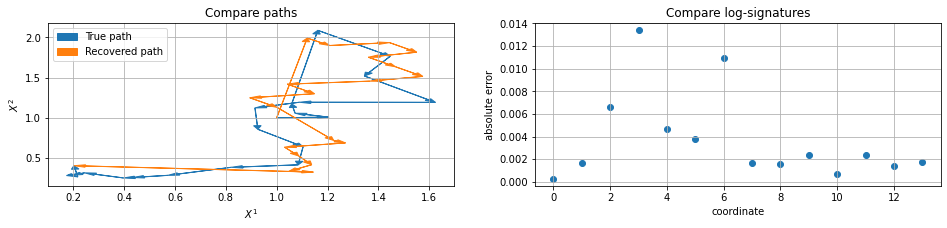
\includegraphics[width=\textwidth]{figs/inverse2.png}
    \caption{Inverse 2-d path with neural method}
\end{figure}
The log-signature error between real path and recovered path are always small by training. But sometimes (frequency like 1 time in 5 experiments) we found that the recovered path is not close to the original one even though their log-signature are very close under $L^{2}$ norm. Possible reasons for this phenomenon follows.
\begin{enumerate}[(i)]
  \item The path embeds tree-like structure so the algorithm does not work in theory. This can be solved by a time augmentation. 
  \item $L^{2}$-error on log-signature space is not a good loss. We can weight different coordinates but there is actually no good reason to do so.
  \item Neural-network is not well designed which produce paths that are too wild and prior on paths space should be added. A more careful study of structure of neural network should be studied in future work.
\end{enumerate}
A direct fix is to apply time augmentation and we perform the numerical comparison below. 
\begin{figure}[H]
  \centering
  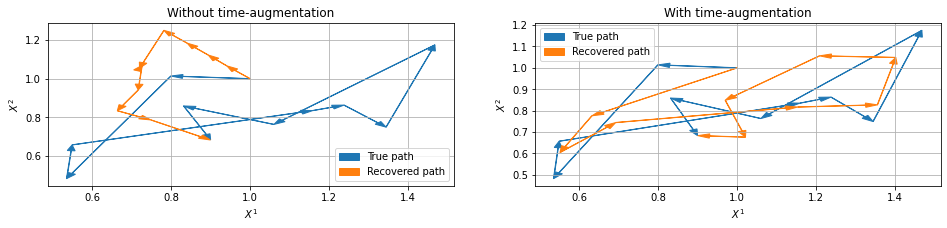
\includegraphics[width=\textwidth]{figs/inverse7.png}
  \caption{Inverse 2-d path with neural method}
\end{figure}
Next, we consider $1$-d path $X_{t} = S^{1}_{t}$ with observation $(X_{i})_{i=0}^{N}$ on $t = \frac{i}{N}$, $i = 0,\cdots N$ and $N = 20$. We apply lead-lag transformation on $(X_{i})_{i=0}^{N}$ which gives a $2$-dimensional path $(\tilde{X}_{i})_{i=0}^{N}$. Then we can use the same procedure above to inverse the log-signature, therefore retrieve the original path. We compare our method with the evolution algorithm by plotting the retrieved path and computing the replication strategy of call option w.r.t the retrieved path. 
\begin{figure}[H]
  \centering
  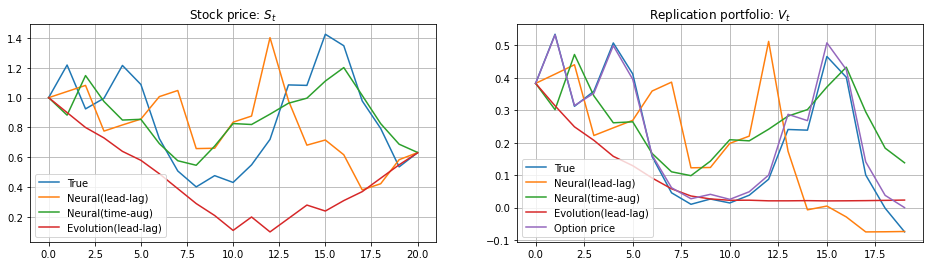
\includegraphics[width=\textwidth]{figs/inverse9.png}
  \caption{Neural method VS evolution algorithm}
\end{figure}
The neural method with lead-lag slightly perform better than the evolution algorithm with lead-lag in most cases, but still sometimes evolution algorithm is better. However, the neural method is much faster! It takes usually $5$ seconds to retrieve a path but evolution algorithm take $5$ minutes. Moreover, we observe that the neural method with time augmentation outperform the other two methods and it is more stable across experiments.   





\section{Path stimulation with signature}
Let us consider numerical stimulations of the following stochastic differential equation
\begin{equation*}
  dX_t = \sum_{k=1}^{m} B^{k}X_{t}dW^{k}_{t},\quad X_{t}\in \mathbb{R}^{n}, W_{t}\in\mathbb{R}^{m}, B^{k} \in \mathbb{R}^{n\times n}
\end{equation*}
where $W_{t}$ is a Brownian motion on $\R^{m}$. We choose $m=n=2$ and 
\begin{equation*}
  B^{1} = \begin{bmatrix}
    0.1& 0.2\\
    0.3& 0.4
  \end{bmatrix},\quad 
  B^{2} = \begin{bmatrix}
    0.4& 0.3\\
    0.2& 0.1
  \end{bmatrix}.
\end{equation*}
Then we stimulate the differential equation by signature 
\begin{equation*}
  \begin{split}
    X_t &= \sum_{d = 0}^{\infty}\sum_{i_{1},\cdots,i_{d} = 1}^{n} \bigg(\int_{0\leq t_{1}\leq\cdots\leq t_{d}\leq t}dW^{i_{1}}_{t_{1}}\cdots dW^{i_{d}}_{t_{d}}\bigg)B^{i_{d}}\cdots B^{i_{1}} X_{0}\\
    &= \sum_{d = 0}^{\infty}\sum_{i_{1},\cdots,i_{d} = 1}^{n} \mathbf{Sig}^{i_{1},\cdots,i_{d}}_{[0,t]}(W) B^{i_{d}}\cdots B^{i_{1}} \cdot X_{0}\\
  \end{split}
\end{equation*}
Here we approximate the signature by growing signature. This is important because if we use higher order, we implicitly assume Stratonovich integral which is not the case here. Or we are using a Milstein scheme and implicitly assume the commutativity of $B^{1}$ and $B^{2}$ here which is also not the case because
\begin{equation*}
  \begin{bmatrix}
    0.1& 0.2\\
    0.3& 0.4
  \end{bmatrix}
  \begin{bmatrix}
    0.4& 0.3\\
    0.2& 0.1
  \end{bmatrix} 
  - 
  \begin{bmatrix}
    0.4& 0.3\\
    0.2& 0.1
  \end{bmatrix}
  \begin{bmatrix}
    0.1& 0.2\\
    0.3& 0.4
  \end{bmatrix}
  = 
  \begin{bmatrix}
    -0.05& -0.15\\
    0.15& 0.05
  \end{bmatrix} \neq 0
\end{equation*} 
Unfortunately, all python packages I know available so far (including esig, iisignature, and Signatory) only support truncated discrete signature. We benchmark with Euler approximation on a very fine grid.
\begin{figure}[H]
    \centering
    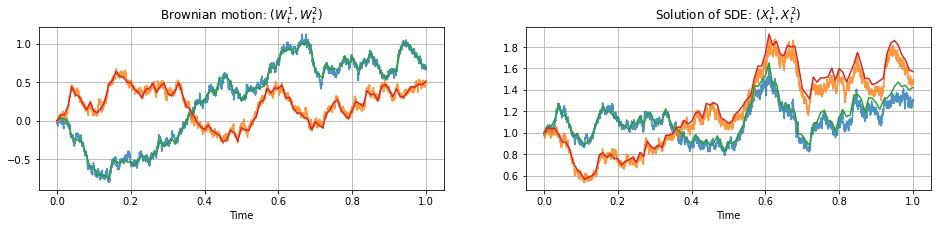
\includegraphics[width=\textwidth]{figs/sde1.png}
    \caption{Solution of SDE stimulated with Euler method on fine grid}
\end{figure}
Below we compare the stimulation between growing discrete signature and truncated discrete signature.
\begin{figure}[H]
    \centering
    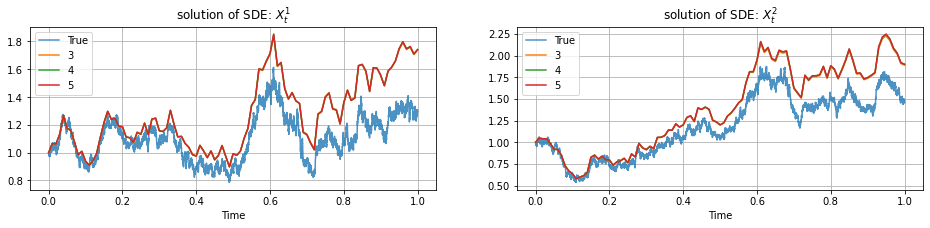
\includegraphics[width=\textwidth]{figs/sde2.png}
    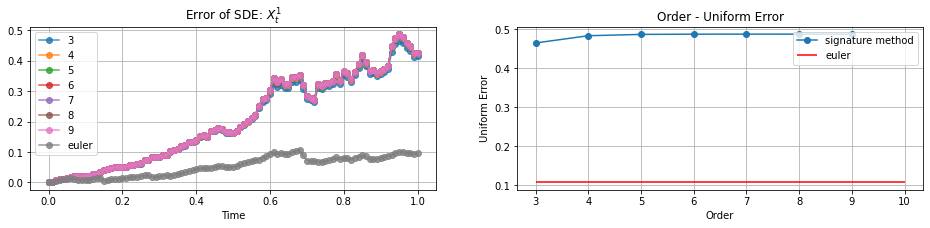
\includegraphics[width=\textwidth]{figs/sde3.png}
    \caption{Truncated discrete signature}
\end{figure}
\begin{figure}[H]
    \centering
    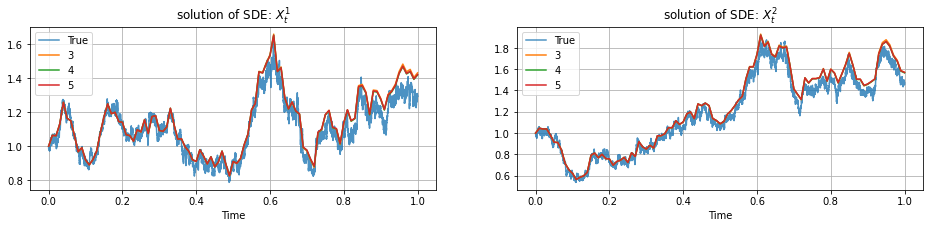
\includegraphics[width=\textwidth]{figs/sde4.png}
    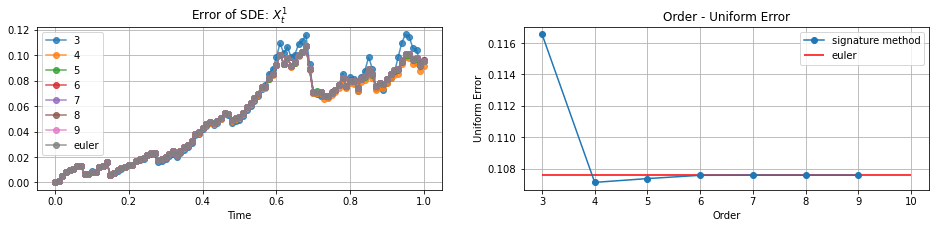
\includegraphics[width=\textwidth]{figs/sde5.png}
    \caption{Growing discrete signature}
\end{figure}
Growing discrete signature outperform the truncated signature. As the order of truncated discrete signature increases, it tends to the limit of approximation with error caused by mis-computing the quadratic variation term. As the order of growing discrete signature increase, the performance tends to the Euler method. This is useful because if we know the signature of our control at $T$, then multiplying the signature with vector field gives a stimulation as good as Euler stimulation running from $0$ to $T$. The key here is the linear relation between signature and the value of SDE. Inversely, this linear relation can be easily learnt by a simple linear regression.

\section{Learning from path to path}
Consider controlled differential equations 
\begin{equation}
  dX_{t} = \sum_{k=1}^{m}V^{k}(X_{t})dW^{k}_{t},\quad X_{t}\in\R^{d}
\end{equation}
By generalized Taylor's expansion we have 
\begin{equation}\label{eq62}
    \begin{split}
        X^{(i)}_{t} &= \sum_{m=0}^{\infty}\sum_{i_{1},\cdots,i_{m} = 1}^{d}\mathbf{Sig}_{[0,t]}^{i_{1},\cdots,i_{m}}(W)\sum_{j=1}^{d}M^{i_{1},\cdots,i_{m}}_{i,j}X^{(j)}_{s}\\
        &= \sum_{m=0}^{\infty}\sum_{i_{1},\cdots,i_{m} = 1}^{d}\sum_{j=1}^{d}M^{i_{1},\cdots,i_{m}}_{i,j} \mathbf{Sig}_{[0s,t]}^{i_{1},\cdots,i_{m}}(W) X^{(j)}_{0}\\
        &= \langle M_{i} ,  \mathbf{Sig}_{[s,t]} \otimes X_{s} \rangle
    \end{split}
\end{equation}
Where $M^{i_{1},\cdots,i_{m}}_{i,j}$ are matrixes depending on $s$. If we let $\mathcal{X} = \mathbf{Sig}_{[s,t]} \otimes X_{s}$ and $\mathcal{Y} = X_{t}$
Therefore, we can learn the relation in \eqref{eq62} by a linear regression on $(\mathcal{X},\mathcal{Y})$. This idea was first shown to me in the machine learning in finance course by Prof. Josef Teichmann, where he also introduced reservoir computing which is closely related to this approach here if you consider the signature stream as a reservoir. We refer interested readers on signature and reservoir computing to ......  Now, we consider $m = d = 2$ and the following dynamic
\begin{equation*}
  V^{1}(X) = \begin{bmatrix}
    2|X^{(2)}|^{0.7}\\
    X^{(2)}
  \end{bmatrix},\quad 
  V^{2}(X) = \begin{bmatrix}
    2|X^{(2)}|^{0.7}\\
    0
  \end{bmatrix},\quad 
  X_{0} = \begin{bmatrix}
    1\\
    2
  \end{bmatrix}.
\end{equation*}
For reservoir space, we consider 
\begin{equation}
  dR_{t} = \sum_{k=1}^{m}(A^{k}R_{t} + b^{k})dW^{k}_{t},\quad R_{t}\in\R^{d}
\end{equation}
where $A^{k}$ and $b^{k}$ are random matrix and vector. We stimulate the real solution $X$ with Euler scheme on $[0,1]$ with $2000$ grid points. 
\begin{figure}[H]
    \centering
    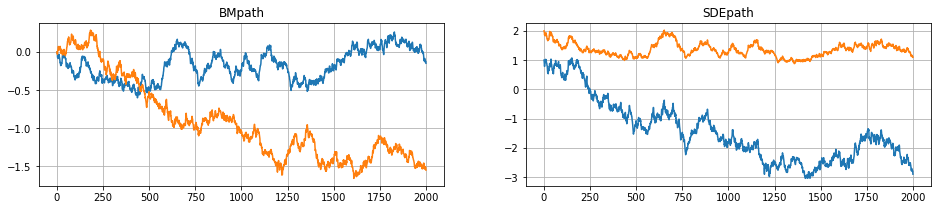
\includegraphics[width=\textwidth]{figs/res1.png}
    \caption{Solution of SDE stimulated with Euler method}
\end{figure}
We choose first $t=1,\cdots 1000$ to be training samples, and $t=1001,\cdots 2000$ to be test samples. We use ridge regression to learn matrixes $M^{i_{1},\cdots,i_{m}}_{i,j}$ on training samples, and generate path on testing samples with learnt matrixes. We compared the generated path with true path under the same random seed. 
\begin{figure}[H]
    \centering
    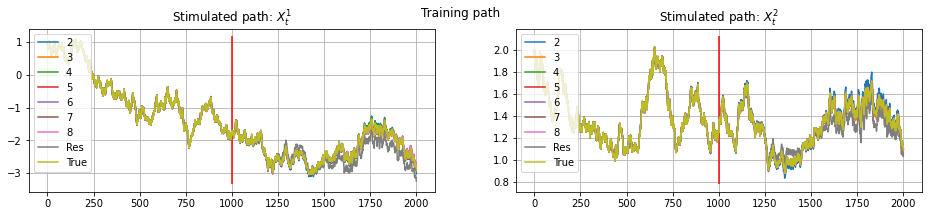
\includegraphics[width=\textwidth]{figs/res2.png}
    \caption{Training path}
\end{figure}
Furthermore, we can generate path starting from $0$ with another random seed $rs$ and compare the generated path with true path under the same random seed $rs$. 
\begin{figure}[H]
    \centering
    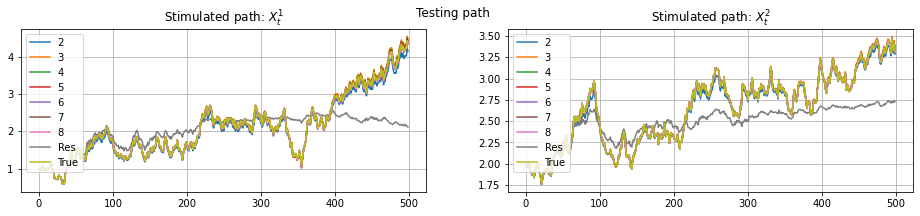
\includegraphics[width=\textwidth]{figs/res3.png}
    \caption{Testing path}
\end{figure}
Now we present the relation between error and order of growing discrete signature 
 \begin{figure}[H]
    \centering
    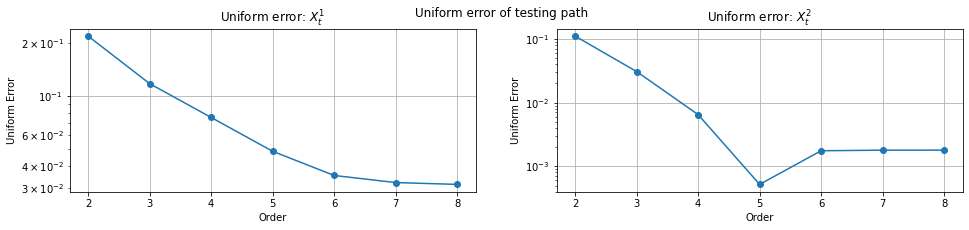
\includegraphics[width=\textwidth]{figs/res4.png}
    \caption{ Order - Error}
\end{figure}
As the order of discrete signature increases, the error decreases and usually touches the limit when order comes to 6. Next, we use generators we just learnt to generate new samples and compared generators based on different truncation order with MMD distance between samples generated by true dynamic. 
\begin{figure}[H]
  \centering
  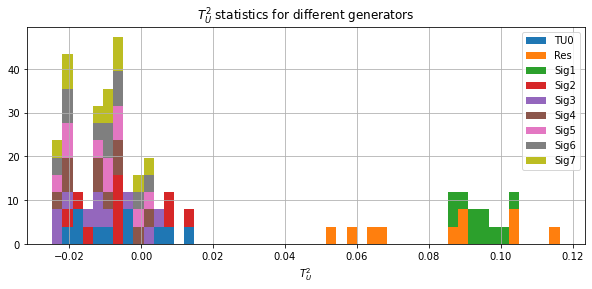
\includegraphics[width=0.8\textwidth]{figs/res5.png}
  \caption{$T_{U}^{2}$ statistics of different generators}
\end{figure}
We found the the market generator learnt by signature of higher order is as good as the real dynamic. In fact, the linear relation not only helps to build a nice model, but contribute to the training procedure because many robust solvers for linear regression are available. If we simply use Adam algorithm to train the same model, the performance is not as good as what we achieved by closed-form solver. 
\begin{figure}[H]
  \centering
  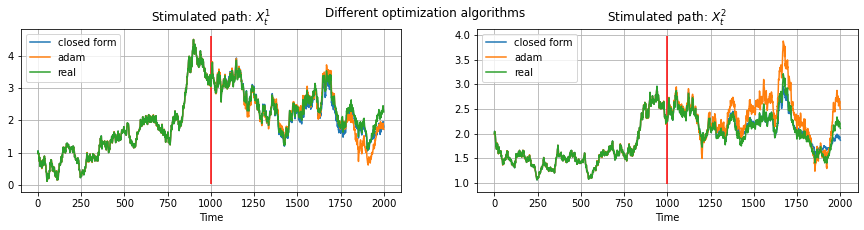
\includegraphics[width=\textwidth]{figs/res6.png}
  \caption{Different optimization algorithms}
\end{figure}
However, it should be pointed out that this linear relation only holds when we consider path starting from the same initial point because matrixes $M^{i_{1},\cdots,i_{m}}_{i,j}$ depends on the gradient of vector field at the starting point $X_{s}$. Therefore, unless the the vector field is linear (gradient independent of $X_{s}$), our model can not be directly applied if samples are paths starting from different initial points. We consider the same controlled differential equation and we split path in to subpaths before construct training data. Since the first dimension is driven by nonlinear dynamic, the performance of training is greatly interfered by splitting data, while even though the second dimension is driven by linear dynamic, the performance still decreases as we split path into subpaths. 
\begin{figure}[H]
  \centering
  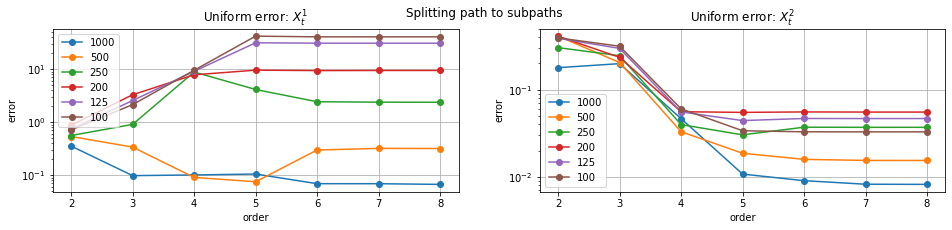
\includegraphics[width=\textwidth]{figs/res7.png}
  \caption{Splitting paths}
\end{figure}
We propose to fix this non-linearity problem by approximate the relation between $X_{s}$ and $M^{i_{1},\cdots,i_{m}}_{i,j}$ by some nonlinear function but more research need to be done in future work. Also, we need to keep in mind that this is not a generative model itself because we are learning the dependency between driving process and controlled process by knowing their value under same random seed. Therefore, in order to generate new samples, we still need to know the distribution of driving process in advance. This might be useful if the target time series you wish to generate is too complicated, but you know that it is driven by some simple process of which you know the distribution. Then, as long as you can observe both the target time series and the simple process, you can apply this methodology to generate new samples.

\chapter{Conclusions and Future Work}


\chapter{Appendix}

\nocite{*}
\bibliographystyle{acm}
\bibliography{workingthesisbib}

\end{document}


 
  